\subsection{Сечение процессов}

Основной задачей данной работы является вычисление сечение реакций
$e^+e^- \to \pi^0 \gamma, \, \eta \gamma$ в доступном диапозоне энергий.
Сечение расчитывается согласно формуле
\begin{equation}
	\sigma = \frac{ N } { L \, (1+\delta_{rad}) \, \varepsilon_{NT} \,
	\varepsilon_{det}} \cdot  
	\left( \frac{ {\varepsilon^{MC}_{\gamma}} }{ {\varepsilon^{exp}_{\gamma}} } \right)^3.
\end{equation}
Здесь $L$ --- интегральная светимость;
$\varepsilon_{det}$ --- эффективность метода, определяется из моделирования;
$\delta_{rad}$ --- радиационная поправка;
$\varepsilon_{NT}$ --- эффективность нейтрального триггера;
вторая дробь соответствует поправке на разницу между моделированием и экспериментом в эффективности
реконструкции фотонов.

Радиационная поправка $\delta_{rad}$ считается по алгоритму, основанному на статье \cite{Kuraev1985}.
Данная поправка является радиационной поправкой к процессам однофотонной аннигиляции $e^+ e^-$-пары,
связанная только с начальным состоянием.
Заявленная точность вычислений не хуже \SI{0.1}{\percent}.
В такую же точность оценивается и вычисление радиационной поправки,
главным образом определяемая алгоритмом аппроксимации сечений интересуемого процесса.
Вычисленные значения $1+\delta_{\text{rad}}$ приведены на рисунке~\ref{fig:rad_corr}.

\begin{figure}[htbp]
	\centering
	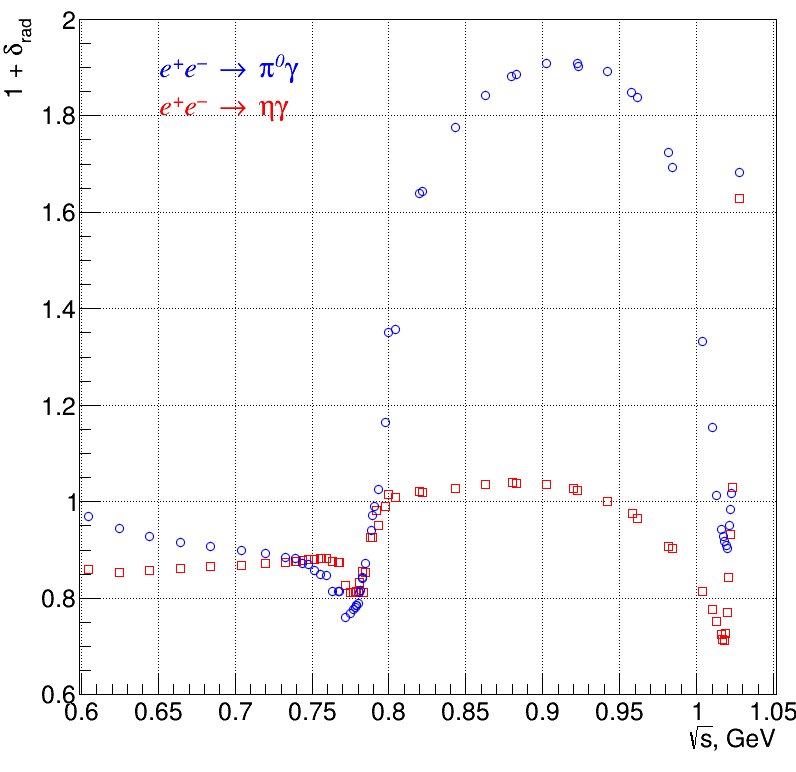
\includegraphics[width=.5\textwidth]{img/rad_corr_for_pseudodisser.png}
	\caption{Радиационная поправка $1+\delta_{\text{rad}}$ для процессов
		$e^+ e^- \to \pi^0 \gamma$ (синие кружки),
		и $e^+ e^- \to \eta \gamma$ (красные квадраты).}\label{fig:rad_corr}
\end{figure}

Инетгральная светимость $L$ на детекторе КМД-3 определяется по процессу Баба рассеяния
$e^+e^- \to e^+e^-$ на большой угол $0.9 < \theta < \pi - 0.9$,
\cite{Ryzhenenkov:2017xqu}.
Достоверность полученных значений контролируется по результатам интгрального сечения $L_{\gamma \gamma}$,
извлекаемого из процесса $e^+e^- \to \gamma \gamma$,
также рассматриваемого в больших углах.
Отличие $1 - L / L_{\gamma \gamma}$ от 0 менее \SI{1}{\percent},
здесь точность ограничено статистикой $e^+e^- \to \gamma \gamma$.

Предварительные результаты по сечения реакций представлены в на рисунках~\ref{fig:cs_pi0g_mine} и~\ref{fig:cs_etag_mine}.

\begin{figure}[htbp]
	\begin{minipage}[t]{.48\textwidth}
		\centering
		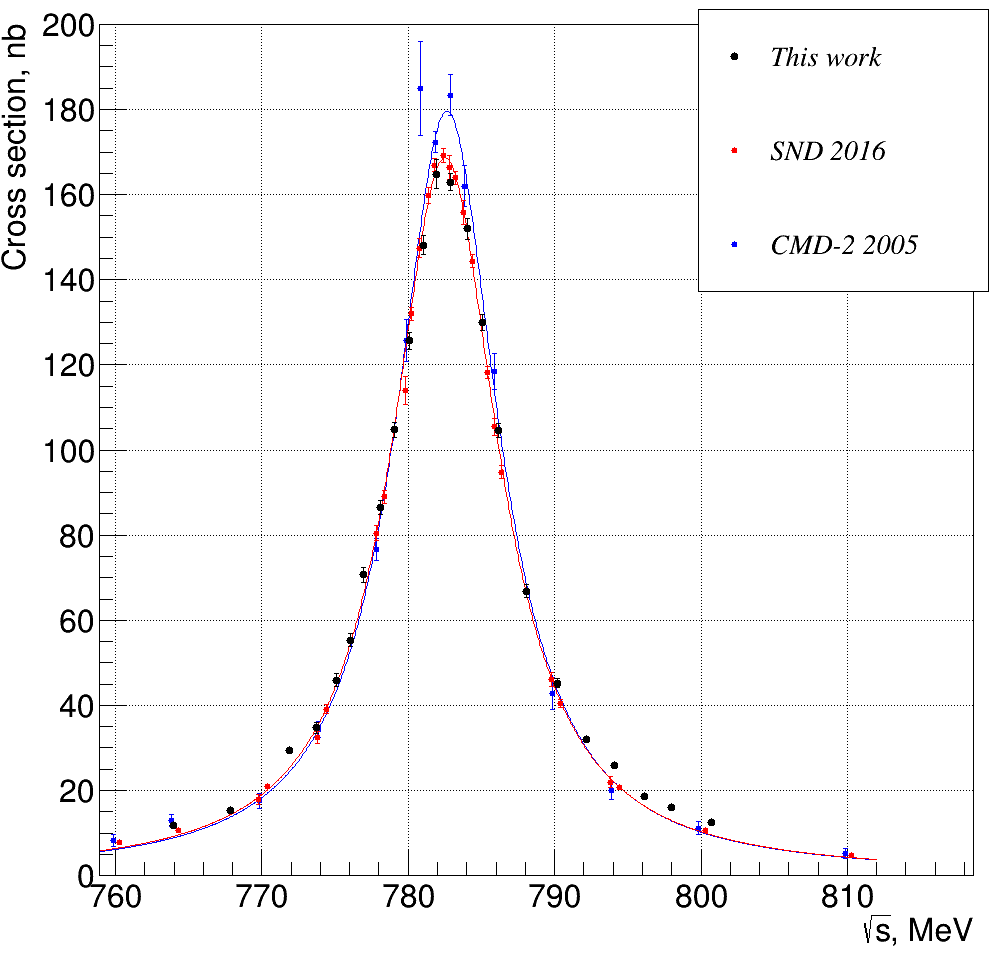
\includegraphics[width=\textwidth]{img/my_pi0g_cross_section_for_pseudodisser.png}
		\caption{Сечение $e^+ e^- \to \pi^0 \gamma$:
			чёрные точки --- предвариетльные результаты данной работы,
			красные (синие) точки и линия --- результаты \cite{Achasov:2016bfr} (\cite{Akhmetshin:2004gw})
			и их аппроксимация нерелятивистк функцией Брейта--Вигнера.}\label{fig:cs_pi0g_mine}
	\end{minipage}
	\hfill
	\begin{minipage}[t]{.48\textwidth}
		\centering
		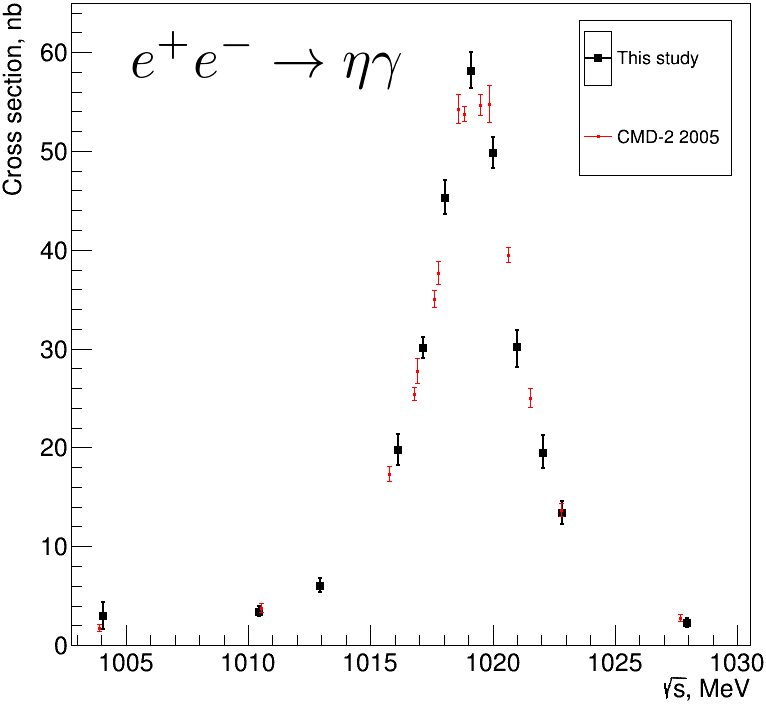
\includegraphics[width=\textwidth]{img/cs_etag_at_phi.png}
		\caption{Сечение $e^+ e^- \to \eta \gamma$:
			чёрные точки --- предвариетльные результаты данной работы,
			красные точки --- результаты \cite{Akhmetshin:2004gw}.}\label{fig:cs_etag_mine}
	\end{minipage}
\end{figure}

%и $e^+e^- \to \gamma \gamma$.%, \cite{lumAkhmetshin2012b}.
%Такой подход позволяет лучше понять и оценить систематические ошибки, которое находятся на уровне \SI{\sim2}{\percent}.
%В ходе определения светимости используются данные моделирования,
%полученные с помощью Монте-Карло генератора фотонных струй (Monte-Carlo Generator Photon Jets)%, \cite{Arbuzov2006}, \cite{Actis2010}),
%модефицированного для изучения продуктов реакций  $e^+e^- \to e^+e^-, \gamma \gamma$.
%Точность расчёта этих сечений с учётом радиационных поправок лучше, чем \SI{0.2}{\percent}.

%Для сравнения полученных сечений с мировыми данными исользованны результаты работ ... .
%Так как данные для процесса $e^+ e^- \to \eta \gamma$ приведенны для различных мод распада $\eta$-мезона,
%то для перевода сечений к одной шкале используются данные %\cite{Beringer:1900zz}.

% \subsubsection{Аппроксимация сечения}